\section{Tema 1: Sucesos y probabilidades}
\subsection{Formalizando}
\begin{defn}[Espacio muestral]
	En un experimento aleatorio, el espacio muestral es el conjunto (no vacío) de sus posibles resultados y se denota por $\Omega$. Puede ser:
	\begin{enumerate}[topsep=1pt, itemsep=1pt,parsep=3pt]
		\item Finito: $\Omega = \{\omega_1, \dots, \omega_N\}$
		\item Infinito numerable: $\Omega = \{\omega_1, \omega_2, \dots\}$
		\item Infinito no numerable, ej.: $\Omega = \left[0, 1\right) \ve \Omega = \mathcal{P}\left(\left[0, 1\right)\right)$
	\end{enumerate}
\end{defn}
\begin{defn}[Espacio de sucesos por Kolmogórov]
	Dado el espacio muestral $\Omega$ de un experimento aleatorio, $\F \subset \mathcal{P}(\Omega)$ es su espcio de sucesos
	\[\iff \left(\F \ne \phi\right) \we \left(A \in \F \implies A^C \in \F\right) \we \left(A_1,A_2, \dots \in \F \implies \bigcup_{j=1}^{\infty} A_j \in \F\right)\]
\end{defn}


\begin{obs}
	De la definición se deduce: \\
	\centerline{
		\begin{itemize*}[itemjoin=\hspace{1cm}]
			\item $\ds \phi \in \F \we \Omega \in \F$
			\item $\ds A_1, \dots, A_n \in \F \implies \bigcup_{j=1}^{n} A_j \in \F$
			\item $\forall A, B \in \F \implies A\cap B \in \F$
		\end{itemize*}
	}
\end{obs}

\begin{defn} [Función o medida de probabilidad]
	Dados espacio muestral $(\Omega)$ y de sucesos $(\F)$ de un experimento aleatorio, la aplicación $\appl{P}{\F}{[0, 1]} : $ es una medida de probabilidad
	\[ \iff \left(P(\Omega) = 1\right) \we \left[P\left(\bigcup_{j=1}^{\infty} A_j\right) = \sum_{j=1}^{\infty} P(A_j) \iff A_i\cap A_j = \phi \tex{ cuando } i \ne j\right] \]
\end{defn}
\begin{prop}
	De la definición se deduce: \\
	\begin{enumerate*}[itemjoin=\hspace{1cm}]
		\item $\ds P\left(\bigcup_{j=1}^n A_j\right) = \sum_{j=1}^{n} P(A_j)$
		\item $\ds P\left(A^C\right) = 1-P(A)$
		\item $\ds P(\phi) = 0$ \\
		\item $\ds P(A\cup B) = P(A) + P(B) - P(A\cap B)$
		\item $\ds A \subseteq B \implies P(A) \leq P(B)$
	\end{enumerate*}
\end{prop}

\begin{ejem}
	En un experimento aleatorio con espacio muestral finito, tomamos \\
	$\ds \Omega = \{\omega_1, \dots, \omega_N\}  \we \F = \mathcal{P} \rightarrow 2^N$. Asignamos $\ds P(\{\omega_j\}) = p_j \we j = 1, \dots, N$ tales que $\ds p_j\geq 0 \we \sum_{j=1}^{N} p_j = 1$. Entonces, $\ds\forall A \in \F : P(A) = \sum_{\omega \in A} P(\omega)$ \\
	\textbf{Caso particular: }$\ds \forall j \in \N_N : p_j = \frac{1}{N} \implies \forall A \in \F : P(A) = \frac{|A|}{N} = \frac{\tex{``Casos favorables''}}{\tex{``Total de casos''}}$
\end{ejem}
\fecha{05/02/2024}
\textbf{Ejemplos varios:}
\begin{enumerate}%[Ejemplos]
	\item (Muy tonto) $\ds\Omega \ne \phi$, tomas $\ds A \subset \Omega : A\ne \phi, \Omega$. \\
	      Dato $\ds p\in (0, 1)$. $\ds\F = \{\phi, A, A^c, \Omega\}$ con $\ds P(A) = p$.
	\item (Bastante general) $\ds\left(\Omega = \{\omega_1, \dots, \omega_N\} \implies |\Omega| = N\right) \we \left(\F = P(\Omega) \rightarrow |\F|=2^N\right)$. \\
	      Dato: $\ds p_1, \dots, p_N \ge 0 \implies \sum_{j=1}^N p_j=1$.
	      Asignamos $\ds \forall j\in \N_N : p_j\defeq P(\{\omega_j\})$.\\
	      Definimos $\ds \forall A\subset \Omega : P(A) = \sum_{\omega \in A}P(\omega)$.\\
	\item Lanzas $n$ veces una moneda. Dato: $p \in (0,1)$.
	      \[\implies \Omega = \{111\cdots1, \dots, 000\cdots0\} \we |\Omega|=2^N \we \tex{escogemos } \F=P(\Omega)\]
	      \[\implies \forall \omega \in \Omega : P(\omega)= p^{\#\tex{unos de }\omega} (1-p)^{\#\tex{ceros de }\omega}\]
	      Comprobamos:
	      \begin{equation*}
		      \begin{split}
			      \ds\sum_{\omega \in \Omega} P(\omega) & =\sum_{k=0}^n \left(\sum_{\substack{\omega\in \Omega                                         \\
			      \#\tex{0s de }\omega = k}} P(\omega)\right)=\sum_{k=0}^n p^k (1-p)^{n-k}\left(|\{\omega\in \Omega :\#\tex{1s de } \omega=k\}|\right) \\
			                                            & =\sum_{k=0}^np^k(1-p)^{n-k} \binom{n}{k} = (p+1-p)^n=1
		      \end{split}
	      \end{equation*}
	\item Lanzamos moneda hasta que sale una cara. Dato $\ds p\in (0,1)$.
	      \[\implies \Omega = \{C, XC, XXC, \dots\} \we \tex{escogemos } \F=P(\Omega)\]
	      \[P(C)\eqdef p \implies P(XC)=p(1-p) \we P(XXC)=p(1-p)^2 \we \dots\]
	      Comprobamos: $\ds\sum_{j=1}^{\infty} p(1-p)^{j-1} = p\sum_{k=0}^\infty(1-p)^k = p \frac{1}{1-(1-p)} = 1$
\end{enumerate}

\subsection{Probabilidad condicionada y total, independencia y Bayes}
Tienes $(\Omega, \F, P)$ y un suceso $A\in \F \rightarrow P(A)$. Llega ``nueva información'': ha ocurrido el suceso $B\in F \longrightarrow$ ¿Debo reasignar la probabilidad de $A$?
\begin{ejem}[Dependencia]
	Lanzas 10 veces una moneda (regular).
	\[A=\{\tex{salen 6 caras}\} \implies P(A)=\frac{\binom{10}{6}}{2^{10}} \approx 20.51 \%\]
	\[B=\{\tex{sale C en 1º}\} \implies P(A)\tex{ sube a }\frac{\binom{9}{5}}{2^9}\]
\end{ejem}

\begin{defn}
	Sea $(\Omega, \F, P)$ un espacio de probabilidad y los sucesos $A, B \in \F : P(B)>0$, $P(A|B)$ es la probabilidad de $A$ condicionada a $B$
	\[\iff P(A|B)=\frac{P(A\cap B)}{P(B)}\]
	\begin{obs}
		En general, $P(A|B)\ne P(B|A)$
	\end{obs}
\end{defn}
\begin{prop}[Cálculo de $P(A|B)$ para cada $A \in \F$]
	Sea $(\Omega, \F, P)$ un espacio de probabilidad y $B \in \F$ un suceso con $P(B)>0$
	\[\implies (\Omega, \F, Q_B) \tex{, con } \appl{Q_B}{\F}{\left[0,1\right]}:Q_B(A)=P(A|B) \tex{, es un espacio de probabilidad}\]
	\begin{dem}
		Basta ver que $Q_B$ es una función de probabilidad.
		\[\left(Q_B(A)=P(A|B)=\frac{P(A\cap B)}{P(B)} \in \left[0, 1\right]\right) \we \left(Q_B(\Omega)=\frac{P(\Omega\cap B)}{P(B)}=\frac{P(B)}{P(B)}=1\right)\]
		Sean $A_1, A_2, \dots \in \F$ disjuntos dos a dos.
		\begin{equation*}
			\begin{split}
				\implies Q_B\left(\bigcup_{j=1}^\infty A_j\right) & =P\left(\bigcup_{j=1}^\infty A_j\;\middle|\; B\right)=\frac{P\left(\bigcup_{j=1}^\infty A_j \cap B\right)}{P(B)}                         \\
				                                                  & =\frac{1}{P(B)}P\left(\bigcup_{j=1}^\infty (A_j \cap B)\right)=\frac{1}{P(B)}\sum_{j=1}^\infty P(A_j\cap B) = \sum_{j=1}^\infty Q_B(A_j)
			\end{split}
		\end{equation*}
	\end{dem}
\end{prop}

\begin{defn}[Independencia]
	Sean $A,B \in \F$ dos sucesos con $P(A), P(B) \geq 0$ son independientes
	\[\iff P(A|B) = P(A) \we P(B|A)=P(B) \textit{ (para entender)}\]
	\[\iff P(A\cap B)=P(A)\cdot P(B) \textit{ (la adecuada)}\]
	\begin{itemize}[topsep=1pt, itemsep=1pt,parsep=3pt]
		\item $A, B$ disjuntos $\implies$ no independientes.
		\item $A_1, \dots, A_N \in \F$ independientes $\ds \iff \forall J \subset \N_N: P\left(\bigcap_{j\in I} A_j\right)=\prod_{j\in J}P(A_j)$ \\
		      $\ds \iff P\left(\overline{A_1}\cap\cdots\cap\overline{A_N}\right)=\prod_{i=1}^N P\left(\overline{A_i}\right)$ donde $\overline{A_i}=A_i, (A_i)^c$
	\end{itemize}
\end{defn}
\begin{ejer}
	Encontrar un espacio de probabilidad en el que haya un conjunto de sucesos independientes dos a dos pero no completamente independientes.
	\[\textbf{SOL: }\Omega = \{1, 2, 3, 4\} \we A=\{1, 2\} \we B=\{2, 3\} \we C=\{1,3\}\]
\end{ejer}

\begin{prop}[Regla de Bayes]
	Sean $(\Omega, \F, P)$ un espacio de probabilidad y $A, B \in \F$ sucesos con $P(A), P(B)>0$
	\[\implies P(A|B)=P(B|A)\cdot \frac{P(A)}{P(B)}\]
	\begin{dem}
		\[P(A|B)=\frac{P(A\cap B)}{P(B)} \we P(B|A)=\frac{P(A\cap B)}{P(A)}\]
		\[\implies P(A|B)\cdot P(B) = P(A\cap B) = P(B|A)\cdot P(A) \implies P(A|B)=P(B|A)\cdot \frac{P(A)}{P(B)}\]
	\end{dem}
\end{prop}

\subsubsection{Probabilidad total}
\begin{prop}
	Sean $(\Omega, \F, P)$ un espacio de probabilidad y $\{B_1, B_2, \dots\}$ una partición de $\ds \Omega : \left(\forall i, j :  i\ne j : B_i\cap B_j = \phi\right) \we \left(\bigcup_{j=1}^\infty B_j=\Omega\right)$
	\[\implies \forall A \in \F : P(A)=P\left(\bigcup_{j=1}^\infty(A\cap B_j)\right)=\sum_{j=1}^\infty(A\cap B_j)=\sum_{j=1}^\infty P(A|B_j)\cdot P(B_j)\]
	\[\implies \forall A \in \F : \boxed{P(A) = \sum_{j=1}^\infty P(A|B_j)\cdot P(B_j)}\]
	\hfill \qedsymbol
\end{prop}
\begin{ejem}
	Sean $U_1=\{10b, 3n\} \we U_2=\{5b, 5n\} \we U_3=\{2b, 6n\}$ tres urnas con bolas blancas ($b$) y negras ($n$). Procedimiento:
	\begin{enumerate}[topsep=1pt, itemsep=1pt,parsep=3pt]
		\item Sorteamos una urna $P(U_1)=\frac{1}{4} \we P(U_2)=\frac{1}{4} \we P(U_3) = \frac{1}{2}$
		\item Sacamos bola de la urna seleccionada.
	\end{enumerate}
	¿Cuál es la probabilidad de que sea blanca?
	\[P(b)=P(b|U_1)P(U_1)+P(b|U_2)P(U_2)+P(b|U_3)P(U_3)\]
\end{ejem}

\begin{ejem}[Peso de la evidencia]
	Sean $U_1=\{80\%\,b, 20\%\,n\} \we U_2=\{20\%\,b, 80\%\,n\}$ dos urnas con bolas blancas ($b$) y negras ($n$). Procedimiento:
	\begin{enumerate}[topsep=1pt, itemsep=1pt,parsep=3pt]
		\item Sorteamos la urna con $\sfrac{1}{2}$ y $\sfrac{1}{2}$ de probabilidad.
		\item Sacamos $10$ bolas (con reemplazamiento).
	\end{enumerate}
	Observamos la evidencia: $bb\dots nb$ ¿qué urna se usó?
	\[P(U_1|5b5n)=P(5b5n|U_1)\frac{P(U_1)}{P(5b5n)}=\frac{P(5b5n|U_1)P(U_1)}{P(5b5n|U_1)P(U_1)+P(5b5n|U_2)P(U_2)}\]
	\[\implies P(5b5n|U_1)=\binom{10}{5}0.8^50.2^5=P(5b5n|U_2) \implies P(U_1|5b5n)=\frac{1}{2}\]
	Este es el resultado que esperábamos, prestemos atención a otro caso más contraintituitivo.
	\[\begin{aligned}
			P(U_1|6b4n) & = \frac{P(6b4n|U_1)P(U_1)}{P(6b4n|U_1)P(U_1)+P(6b4n|U_2)P(U_2)}                                                                                   \\
			            & = \frac{\binom{10}{6}0.8^60.2^4\cdot\sfrac{1}{2}}{\binom{10}{6}0.8^60.2^4\cdot\sfrac{1}{2} + \binom{10}{6}0.8^40.2^6\cdot\sfrac{1}{2}}\approx90\%
		\end{aligned}\]
\end{ejem}
\begin{wrapfigure}{r}{4.3cm}
	\includesvg[width=4cm]{img/graph1.svg}
\end{wrapfigure}

Si dibujamos la gráfica de la función \[ f(x)=P(U_1 | xb(10-x)n)\] podemos ver que el cambio es muy brusco. Es decir, una pequeña diferencia en la evidencia puede cambiar mucho la probabilidad de que se haya usado una urna u otra.



\begin{ejem}[Falsos positivos/negativos]
	Hay una enfermedad $(E \ve S)$ y hay una prueba para detectar $(+ \ve -)$. Datos: $P(+ | E)=95\% \we P(-| S)=99\%$.\\
	Te haces la prueba y sale $+$:
	\[P(E|+)=P(+|E)\frac{P(E)}{P(+)}=\frac{P(+|E)P(E)}
		{P(+|E)P(E)+P(+|S)P(S)}\]
	Conozco todas estas probabilidades excepto $p\defeq P(E) \implies P(S)=1-p$.
\end{ejem}
\begin{wrapfigure}{l}{3.2cm}
	\vspace{-0.85cm}
	\includesvg[width=3cm]{img/graph2.svg}
\end{wrapfigure}
Si definimos $f(p)\defeq P(E|+)$ \[\implies \{f(0.5)=98.95\% \we f(\sfrac{1}{100}) = 48.97\%\we f(\sfrac{1}{1000}) = 8.68\% \}\]
Es decir, si la incidencia es muy baja, no tiene sentido hacer pruebas masivamente porque la mayoría de positivos serán falsos.

\begin{ejem}[Sobre independencia]
	$(\Omega, \F, P) \we A_1, \dots, A_n$ sucesos independientes tal que $\forall j \in \N_n : P(A_j)=\frac{1}{n}$. ¿Qué sabemos sobre $\ds P\left(\bigcup_{j=1}^n A_j\right)$?
	\[\tex{En general, sabemos que } \frac{1}{n}\leq P\left(\bigcup_{j=1}^n A_j\right) \leq \sum_{j=1}^nP(A_j)\leq 1\]
	$n=2$: $\ds P(A\cup B)=P(A)+P(B)-P(A\cap B)=\sfrac{3}{4}$ \\
	$n=3$: $\ds P(A\cup B\cup C)=\binom{3}{1}\frac{1}{3}-\binom{3}{2}\frac{1}{3^2}+\binom{3}{3}\frac{1}{3^3}=\sfrac{19}{27}$ \\
	$n$ general: $\ds P\left(\bigcup_{j=1}^n A_j\right)=\sum_{j=1}^nP(A_j)-\sum_{1\leq i<y\leq n} P(A_i\cap A_j) + \cdots$ (Inclusión exclusión)
	\[\implies P\left(\bigcup_{j=1}^n A_j\right)= \binom{n}{1}\frac{1}{n} - \binom{n}{2}\frac{1}{n^2} + \binom{n}{3}\frac{1}{n^3} + \cdots=\sum_{j=1}^n\binom{n}{j}\frac{1}{n^j}(-1)^{j+1}\]
	\[\implies P\left(\bigcup_{j=1}^n A_j\right)= 1-\sum_{j=0}^n\binom{n}{j}\left(\frac{-1}{n}\right)^j=1-\left(1-\frac{1}{n}\right)^n\xrightarrow{n\rightarrow\infty}1-\frac{1}{e}\]
\end{ejem}

\subsubsection{Continuidad de la probabilidad: detalle técnico}

\begin{prop}
	Sean $(\Omega, \F, P)$ un espacio de probabilidades y $ A_1, \dots : A_1 \subset A_2 \subset \cdots$ una sucesión creciente de conjuntos
	\[\implies P\left(\bigcup_{j=1}^\infty A_j\right)=\lim_{n\rightarrow\infty}P\left(A_n\right)\]
	\begin{dem}
		Se trata de describir $\bigcup_{j=1}^n A_j$ como la unión de conjuntos disjuntos.
		\[P\left(\bigcup_{j=1}^n A_j\right)=P\left(A_1\cup\bigcup_{j=1}^{n-1} \left(A_{j+1}\setminus A_j\right)\right)=P(A_1)+\sum_{j=1}^{n-1}\left(P(A_{j+1})-P(A_j)\right)=P(A_n)\]
		\[\implies P\left(\bigcup_{j=1}^\infty A_j\right) = P(A_1)+\sum_{j=1}^{\infty}\left(P(A_{j+1})-P(A_j)\right)=\lim_{n\rightarrow\infty}P(A_n)\]
	\end{dem}
\end{prop}

%12/02/2024
\begin{prop}
	Si la sucesión $A_1, \dots$ es decreciente
	$\ds\implies P\left(\bigcap_{j=1}^\infty A_j\right)=\lim_{n\rightarrow\infty}P\left(A_n\right)$
\end{prop}

\begin{teo}[Continuidad de la probabilidad]
	En el espacio de probabilidades $(\Omega, \F, P)$, sea $A_1, A_2, \dots$ una sucesión $: \forall j \in \N : A_j \in \F$
	\[\implies P\left(\bigcup_{j=1}^\infty A_j\right)=\lim_{n\rightarrow\infty}P\left(\bigcup_{j=1}^n A_j\right)\]
	\begin{dem}
		Definimos $\ds B_i\defeq\bigcup_{j=1}^i A_j \implies \bigcup_{j=1}^\infty A_j = \bigcup_{i=1}^\infty B_i \we (B_i)$ es creciente.
		\[\implies P\left(\bigcup_{j=1}^\infty A_j\right) = P\left(\bigcup_{i=1}^\infty B_i\right) = \lim_{n\rightarrow\infty}P\left(B_n\right)=P\left(\bigcup_{j=1}^n A_j\right)\]
	\end{dem}
\end{teo}

\subsection{Variables aleatorias (discretas)}
\begin{defn}
	Sea $(\Omega, \F, P)$ un espacio de probabilidades, $\appl{X}{\Omega}{\R}$ es una variable aleatoria discreta* (v.a.d.)
	\[\iff \tex{(1) } X(\Omega) \tex{ es numerable*} \we \tex{ (2) }\forall x \in \R : \{\omega \in \Omega : X(\omega)=x\} \in \F\]
	En realidad, solo interesa (2) cuando $x=x_j$
\end{defn}
\begin{defn}
	Sea $X$ una v.a.d. en $(\Omega, \F, P)$, $\appl{p_X}{\R}{\left[0,1\right]}$ es su función de masa
	\[\iff x\longmapsto p_X(x)=P(X=x)\defeq P(\{\omega \in \Omega : X(\omega)=x\})\]
	Vemos que
	\[\sum_{j\geq1}p_X(x_j)=\sum_{j\geq1}P(X=x_j)=\sum_{j\geq1} P(\{\omega \in \Omega : X(\omega)=x_j\})=P\left(\bigcup_{\omega\in\Omega}\{\omega\}\right)=P(\Omega)=1\]
	Lo relevante es el conjunto de posibles valores de $X$ $(\{x_1, x_2, \dots\})$ numerable y el conjunto (también numerable) de probabilidades $\{p_1, p_2, \dots\}$ donde
	\[\bigg(\forall j \geq 1 : p_j=P(x=x_j) \we p_j\geq 0 \bigg) \we \sum_{j\geq 1}p_j=1\]
\end{defn}

%13/02/2024
\begin{teo}
	Sea $S=\{x_1, x_2, \dots \}$ un conjunto y $(\Pi_1, \Pi_2, \dots, \Pi_j)$ una lista tal que \\
	$\forall i \leq j : \Pi_i \geq 0 \we \sum_{j\geq 1}\Pi_j=1$
	\[\implies \exists (\Omega, \F, P) \we X\tex{ v.a.d }:\big(\forall  x\notin S :p_X(x)= 0 \big) \we p_X(x_i)=\Pi_i\]
	\begin{dem}
		Fijamos $\Omega = S$ y $\F=\mathcal{P}(S)$.
		\[A\in \F \implies P(A)=\sum_{j:x_j\in A}\Pi_j \we X(x_j)=x_j\]
	\end{dem}
\end{teo}

\begin{ejem}[Diferentes modelos de distribución de probabilidad]
	\begin{enumerate}
		\item []
		\item $X$ sigue una distribución \textbf{uniforme} en $\{1, \cdots, N\}, N\geq2$ $(X\sim\unif{N})$.
		      \[\iff S=\{1, \cdots, N\} \we {\Pi_j}={\sfrac{1}{N}, \dots, \sfrac{1}{N}}\]
		      Se usa para modelizar un lanzamiento de un dado regular de $N$ caras.
		\item $X$ sigue una distribución de \textbf{Bernoulli} con parámetro $p$ ($X\sim\ber{p}$)
		      \[\iff \begin{cases}
				      p_X(x)=0 \iff x\ne 0, 1 \\
				      p_X(1)=p \we p_X(0)=1-p
			      \end{cases}\iff\begin{cases}
				      P(X=1)=p \\
				      P(X=0)=1-p
			      \end{cases}\]
		      donde $1$ es éxito y $0$ fracaso. Se usa para modelizar el resultado de un experimento con dos posibles resultados, i.e. una moneda no necesariamente regular.
		\item $X$ sigue una distribución \textbf{binomial} de parámetros $n\geq 1 \we p\in (0, 1)$ ($X\sim\bin{n, p}$)
		      \[\iff S=\{0, 1, \dots, n\} \we \forall j\in \{0, 1, \dots, n\}:P(x=j)=\binom{n}{j}p^j(1-p)^{n-j}\]
		      Sirve para modelizar el número de caras que salen al lanzar $n$ veces una moneda de probabilidad $p$.
		      \[n! \sim n^ne^{-n}\sqrt{2\pi n}\implies \binom{n}{\sfrac{n}{2}}\sim\frac{n^ne^{-n}\sqrt{2\pi n}}{(\sfrac{n}        {2})^{(\sfrac{n}{2})}e^{-(\sfrac{n}{2})}\sqrt{2\pi (\sfrac{n}{2})}(\sfrac{n}{2})^{(\sfrac{n}{2})}e^{-(\sfrac{n}     {2})}\sqrt{2\pi (\sfrac{n}{2})}}\]

		      \[\implies \frac{n^n\sqrt{n}}{(\sfrac{n}{2})^{(\sfrac{n}{2})}\sqrt{2\pi (\sfrac{n}{2})}(\sfrac{n}{2})^{(\sfrac{n}       {2})}\sqrt{(\sfrac{n}{2})}} =
			      \frac{n^n\sqrt{n}}
			      {(\sfrac{n}{2})^{n}\sqrt{2\pi}(\sfrac{n}        {2})}=\frac{n^n\sqrt{2}}{(\sfrac{n}{2})^n\sqrt{\pi      n}}=2^n\sqrt{\frac{2}{\pi n}}\]
		\item La variable $X$ sigue una distribución \textbf{geométrica} de parámetro $p\in(0,1)$ ($X\sim\geom{p}$).
		      \[\iff S=\{1, 2, \dots\} \we \forall j \geq 1 : P(x=j)=p(1-p)^{j-1}\]
		      Sirve para modelizar el número de lanzamientos hasta que sale un resultado $C$ en cuestión con $P(X=C)=p$. \vspace{-0.3cm}
		      \begin{obs}
			      Cuidado porque existen variables aleatorias que también se dicen de distribución geométrica en las que $S=\{0, 1, 2, \dots\}$. Se habla de cuantas veces has obtenido el resultado complementario a $C$ antes de que halla salido $C$.
		      \end{obs}
		\item La variable $X$ sigue una distribución de \textbf{Poisson} con parámetro $\lambda>0$ ($X\sim \poisson{\lambda}$)
		      \[\iff S=\{0, 1, \dots\} \we \forall j \geq 0 : P(x=j)=e^{-\lambda}\frac{\lambda^j}{j!}\]
		      Se usa para modelizar la frecuencia de eventos determinados durante un intervalo de tiempo fijado a partir de la frecuencia media de aparición de dichos eventos.
	\end{enumerate}
\end{ejem}

\begin{prop}
	Sea $X\sim \bin{n, p}$ una v.a.d.
	\[\implies \tex{cuando $n$ es grande, }\bin{n, p}\sim\poisson{np}\]
	\begin{dem}
		Fijo $\ds\lambda>0 \we p=\frac{\lambda}{n}$.
		\[\lim_{n\rightarrow\infty} \binom{n}{k}\frac{\lambda^k}{n^k}\left(1-\frac{\lambda}{n}\right)^{n-k}=\frac{\lambda^k}{k!}\lim_{n\rightarrow\infty} \frac{n!}{(n-k)!}\frac{1}{n^k}\left(1-\frac{\lambda}{n}\right)^n\left(1-\frac{\lambda}{n}\right)^{-k}=e^{-k}\frac{\lambda^k}{k!}\]

	\end{dem}
\end{prop}

\begin{ejem}[¿Hay más ejemplos?] \mbox{} \\
	\begin{itemize*}[itemjoin=\hspace{1cm}]
		\item Binomial negativa
		\item Hipergeométrica \\
		\item Dada cualquier serie convergente $\ds \sum_{n=1}^\infty a_n = s$, se puede definir la variable aleatoria $X$ tal que $\ds S=\{1, 2, \dots\} \we P(x=k)=\frac{a_k}{s}$
	\end{itemize*}
\end{ejem}

\subsubsection{Funciones transformadoras de variables aleatorias (discretas)}
Sea $X$ una v.a.d. y $\appl{g}{\R}{\R}$ una función, definimos $Y\defeq g(X)$.
\[\implies \{\omega \in\Omega:Y(\omega)=g(X(\omega))=y\} \in \F \implies Y\tex{ es una v.a.d}\]
Por otro lado,
\[\forall y \in \R:P(Y=y)=P(g(X)=y)=P(X\in g^{-1}(y))=\sum_{x\in g^{-1}(y)}P(X=x)=\sum_{x\in g^{-1}(y)}p_X(x)\]

\begin{ejem}[$Y=x^2$]
	$$p_Y(y) = P(Y=y)=P(X^2=y)=\begin{cases}
			0,                                                                              & y <0 \\
			P(X=0)=p_X(0),                                                                  & y=0  \\
			P\left(X=\pm\sqrt{y}\right)=p_X\left(\sqrt{y}\right)+p_X\left(-\sqrt{y}\right), & y>0
		\end{cases}$$
\end{ejem}

\subsubsection{Resúmenes: esperanza, varianza, momentos}

\begin{defn}[Esperanza]
	Sea $X$ una v.a.d. en el espacio de probabilidad $(\Omega, \F, P)$ y con función de masa $p_X$, $E(X)$ es la esperanza de $X$ (también llamada media o \emph{expectatio})
	\[\iff E(X)=\sum_{x\in X(\Omega)}x\cdot P(X=x)=\sum_{j\geq 1}x_j\cdot p_X(x_j)\]
	Pero ojo, solo si la serie es absolutamente convergente.
	\[\begin{cases} \tex{Si $x_1, \dots, x_N$ finito, la suma obviamente converge.} \\
			\tex{Si los $x_j$ son positivos, la serie converge si y solo si es acotada. Si no lo es diverge a $\infty$.}\end{cases}\]
\end{defn}

\begin{ejem}[Cálculo de la esperanza]
	\begin{itemize}[topsep=1pt, itemsep=1pt,parsep=3pt]
		\item[]
		\item $\ds x_1, \dots, x_N \we p_1, \dots, p_N \implies E(X)=\sum_{j=1}^N x_j\cdot p_j$
		\item $\ds X\sim\ber{p} \implies E(X)=1\cdot p+0\cdot(1-p)\implies \boxed{E(X)=p}$
		\item $\ds X\sim\unif{1, \dots, N} \implies E(X)=\frac{1}{N}\sum_{n=1}^N n \implies \boxed{E(X)=\frac{N+1}{2}}$
		\item $\ds X\sim\bin{n, p} \implies E(X)=\sum_{j=0}^n j\binom{n}{j}p^j(1-p)^{n-j}\implies \boxed{E(X)=np}$ \\
		      Se obtiene derivando el binomio de Newton $\ds (1+x)^n=\sum_{j=0}^n \binom{n}{j} x^j$
		      \[\implies \odv{}{x}(1+x)^n=\sum_{j=0}^n \binom{n}{j} j\cdot x^{j-1} \implies xn(1+x)^{n-1}=\sum_{j=0}^n \binom{n}{j} jx^{j}\]
		      Si $\ds x=\frac{p}{1-p} \implies \frac{p}{1-p}n\left(1+\frac{p}{1-p}\right)^{n-1}=\sum_{j=0}^n \binom{n}{j} j\left(\frac{p}{1-p}\right)^{j}$
		      \[\implies \frac{p}{1-p}n\left(\frac{1}{1-p}\right)^{n-1}=\sum_{j=0}^n \binom{n}{j} j\left(\frac{p}{1-p}\right)^{j}\]
		      \[\implies np=(1-p)^n\sum_{j=0}^n \binom{n}{j} j\left(\frac{p}{1-p}\right)^{j} = \sum_{j=0}^n j\binom{n}{j}p^j(1-p)^{n-j} = E(X)\]
		      \hfill \qedsymbol
		\item $X\sim \geom{p}$ $\ds \implies E(X)=\sum_{k=1}^\infty k\cdot p\cdot(1-p)^{k-1} \implies \boxed{E(X)=\frac{1}{p}}$
		      \[\forall  x :\abs{x}<1: \frac{1}{1-x}=\sum_{n=0}^\infty x^n\implies \frac{1}{(1-x)^2}=\sum_{n=1}^\infty nx^{n-1}\implies E(X)= p \frac{1}{p^2}=\frac{1}{p}\]
		      \hfill \qedsymbol
		\item $\ds X\sim\poisson{\lambda} \implies E(X)=\sum_{j=0}^\infty j\frac{\lambda^j}{j!}e^{-\lambda}\implies \boxed{E(X)=\lambda}$
		      \[\implies E(X)=e^{-\lambda}\lambda\sum_{k=1}^\infty \frac{\lambda^{k-1}}{(k-1)!}=\lambda e^{-\lambda}\sum_{j=0}^{\infty} \frac{\lambda^j}{j!}=\lambda\]
		      \hfill \qedsymbol
	\end{itemize}
\end{ejem}

\begin{ejem}
	Sea $X$ una v.a.d. con $\ds \forall k \geq 0 : P(X=k)=\frac{6}{\pi^2}\frac{1}{k^2}$
	\[\implies E(X)=\sum_{k=1}^\infty k\frac{6}{\pi^2}\frac{1}{k^2}=\frac{6}{\pi^2}\sum_{k=1}^\infty \frac{1}{k} \tex{  que diverge a } \infty\]
\end{ejem}
\begin{ejem}
	Sea $X$ una v.a.d. que toma valores en $\{(-1)^{k+1}k : k \geq 1\} = \{1, -2, 3, -4, \dots\}$
	\[P(X=(-1)^{k+1}k)=\frac{6}{\pi^2}\frac{1}{k^2} \implies E(X)=\sum_{k=1}^\infty \frac{(-1)^{k+1}}{k} \tex{ que sabemos que tiende a } \ln{2}\]
	Sin embargo, la serie no converge absolutamente, por tanto, mediante argumentos de reordenación, se puede argumentar que $E(X)$ toma cualquier valor real. Entonces $E(X)$ no tiene sentido.
\end{ejem}

\begin{teo} \label{teo:esperanzaporg}
	Sea $X$ una v.a.d. que toma los valores $x_j$ con probabilidades $p_j$ para $j \geq 1$. Sea $\appl{g}{\R}{\R}$ una función.
	\[\implies E(g(X))=\sum_{j\geq 1}g(x_j)p_j\]
	\begin{dem}
		Sabemos que $g(X)$ es una v.a.d. que toma valores en $\{g(x_j) : j\geq 1\}$, donde $\abs{\{g(x_j)\}}\leq\abs{\{x_j\}}$ porque $g$ puede no ser inyectiva. \\
		Como $\ds P(g(X)=y) = \sum_{x\in g^{-1}(y)} P(X=x)$
		\[\implies E(g(X))=\sum_{y\in g(X(\Omega))}y\cdot P(g(X)=y)=\sum_{y\in g(X(\Omega))}y \left(\sum_{x\in g^{-1}(y)} P(X=x)\right)\]
		Como $\ds \forall y \in g(X(\Omega)) : \exists \, \abs{g^{-1}(y)} \tex{ cantidad de } i_\tex{s} \geq 1 : g(x_i)=y$ se tiene
		\[E(g(X))=\sum_{j\geq 1}g(x_j)p_j\]
	\end{dem}
\end{teo}

\begin{obs}
	\begin{enumerate}
		\item[]
		\item Si $X$ es tal que $P(X=a)=1\implies E(X)=a$
		\item $X \sim \unif{\{-1, 0, 1\}} \we Y=X^2 \implies E(X)=0 \we E(Y)=\sfrac{2}{3}$
		\item $E(aX+b)=aE(X)+b$ porque
		      \[\sum_{j\geq 1}(ax_j+b)p_j=a\sum_{j\geq 1}x_jp_j+b\sum_{j\geq 1}p_j=aE(X)+b\]
		\item En general $E(g(X)) \ne g(E(X))$ \hfill \textbf{(Motivo de excomunión)}
		      \begin{ejem}[$X\sim\poisson{\lambda} \implies E(X)=\lambda$]
			      Si $Y=g(X)=e^X$
			      \[\implies E(Y)=E(e^Y)=\sum_{j=0}^\infty e^j\frac{\lambda^j}{j!}e^{-\lambda}=e^{-\lambda}\sum_{j=0}^\infty \frac{(e\lambda)^{j}}{j!}=e^{-\lambda}e^{e\lambda}=e^{\lambda(e-1)}\ne e^\lambda\]
		      \end{ejem}
	\end{enumerate}
\end{obs}

\begin{defn}[Varianza]
	Sea $(\Omega, \F, P)$ un espacio de probabilidad y $X$ una v.a.d. con función de masa $p_X$, $V(X)$ es la varianza de $X$
	\[\iff V(X)=E\left[(X-E(X))^2\right]\]
	Si $X$ toma valores $x_1, x_2, \dots$ con probabilidades $p_1, p_2, \dots$ y denominamos $\mu \defeq E(X)$
	\[\implies V(X)=\sum_{j\geq 1}(x_j-\mu)^2\cdot p_j = \sum_{j\geq 1}(x_j-\mu)^2\cdot p_j = \sum_{j\geq 1}(x_j^2-2x_j\mu+\mu^2)\cdot p_j\]
	\[\implies V(X)=\sum_{j\geq 1}x_j^2p_j -2\sum_{j\geq 1}x_j\mu p_j +\sum_{j\geq 1}\mu^2p_j = E(X^2)-2\mu^2+\mu^2\]
	\[\implies \boxed{V(X) = E\left[\left(X-E(X)\right)^2\right] = E\left(X^2\right)-{E(X)}^2}\]
\end{defn}

\begin{obs}
	\begin{enumerate}
		\item[]
		\item $V(X)$ es medida de dispersión de $X$ alrededor de $E(X)$.
		\item $V(X)\geq 0$
		\item $V(X)=0\implies P(X=E(X))=1$
		\item $\lbox{V(aX+b)}=E[(aX+b-E(aX+b))^2]=E\left[(aX-aE(X))^2\right]=\rbox{a^2V(X)}$
		\item Las unidades de $V(X)$ son las de $X^2$ \[\implies \tex{definimos la desviación típica de $X$ como } \boxed{\sigma(X)\defeq\sqrt{V(X)}}\]
		\item ¿Por qué no $E(|X-E(X)|)$? \\
		      Porque el valor absoluto no es diferenciable y no se puede trabajar con él.
	\end{enumerate}
\end{obs}

\begin{ejem}
	\begin{enumerate}
		\item[]
		\item $\ds X\sim\ber{p} \implies E(X)=p \we \lbox{V(X)}=p-p^2=\rbox{p(1-p)}$
		\item $\ds X\sim \unif{\{1, \dots, N\}} \implies E(X)=\frac{N+1}{2} \we \boxed{V(X)=\frac{N^2-1}{12}}$
		      \[\implies V(X)=\frac{1}{N}\sum_{j=1}^N j^2=\frac{1}{N}\cdot\frac{N(N+1)(2N+1)}{6}=\frac{(N+1)(N-1)}{12}\]
		\item $\ds X\sim\bin{n, p} \implies E(X)=np \we \boxed{V(X)=np(1-p)}$
		      \begin{dem}

		      \end{dem}
		\item $\ds X\sim\geom{p} \implies E(X)=\frac{1}{p} \we \boxed{V(X)=\frac{1-p}{p^2}}$
		      \begin{dem}

		      \end{dem}
		\item $X\sim\poisson{\lambda} \implies E(X)=\lambda \we \boxed{V(X)=\lambda}$
		      \begin{dem}
			      \[E(X^2)=\sum_{k=0}^{\infty} k^2 e^{-k}\frac{\lambda^k}{k!}\]
		      \end{dem}
	\end{enumerate}
\end{ejem}

\begin{defn}[Momentos de $X$]
	Sea $X$ una v.a.d. con función de masa $p_X$, $\mu_k$ es el \textbf{$k$-ésimo momento} de $X \iff \mu_k= E\left[(X-E(X))^k\right]$
\end{defn}

\begin{obs} Algunos momentos tienen nombre propio: \\
	\begin{enumerate*}[itemjoin=\hspace{1cm}]
		\item $\mu_1=0$
		\item $\mu_2=V(X)$
		\item $\mu_3$ es la \textbf{asimetría} de $X$
		\item $\mu_4$ es la \textbf{curtosis} de $X$
	\end{enumerate*}
\end{obs}

\begin{teo}[Desigualdad de Markov]
	Sea $X$ una v.a.d. $: P(X<0)=0 \we E(X)<\infty$
	\[\implies \forall t >0 : P(X\geq t) \leq \frac{E(X)}{t}\]
	\begin{dem}
		\textbf{Notación:} En $(\Omega, \F, P)$, $A\subset \F$ y $\ds \mathbbm{1}_A(\omega) = \begin{cases}
				1 \tex{ si } \omega \in A \\
				0 \tex{ si } \omega \notin A
			\end{cases}$ \\
		Fijamos $t>0$ y definimos $Y_t(\omega)=t\cdot \mathbbm{1}_{\{x\geq t\}}(\omega)=\begin{cases}
				t \tex{ con probabilidad } P(x\geq t) \\
				0 \tex{ con probabilidad } 1-P(x\geq t)
			\end{cases}$
		\[\implies \forall \omega : Y_t(\omega)\leq X(\omega) \implies E(Y_t)=t\cdot P(X\geq t)\leq E(X)\]
		Así que $\ds \forall t >0 : P(X\geq t) \leq \frac{E(X)}{t}$
	\end{dem}
\end{teo}

\begin{teo}[Desigualdad de Chebyshev]
	Sea $X$ una v.a.d. $: E(X), V(X)< \infty$.
	\[\implies \forall \lambda>0 : P(|X-E(X)|\geq \lambda\cdot \sigma(X)) \leq \frac{1}{\lambda^2}\]
	\[\iff \forall \alpha > 0 : \boxed{P\left(|X-E(X)|\geq \alpha\right) \leq \frac{V(X)}{\alpha^2}}\]
	\begin{dem}
		Definimos $Y=|X-E(X)|^2$ y aplicamos la desigualdad de Markov.
		\[\implies \forall t > 0 : P(Y\geq t) \leq \frac{E(Y)}{t} \implies \forall t>0: P(\abs{X-E(X)}^2\geq t)\leq \frac{E(Y)}{t}\]
		\[\tex{Como } E(Y) = E(|X-E(X)|^2) = V(X) \tex{ por la def de varianza,}\]
		\[\implies \forall t>0: P\left(|X-E(X)|\geq \sqrt{t}\right)\leq \frac{V(X)}{t}\]
		Definimos $\ds \alpha\defeq \sqrt{t} \implies \forall \alpha>0: P\left(|X-E(X)|\geq \alpha\right)\leq \frac{V(X)}{\alpha^2}$\\
		y para la desigualdad equivalente definimos $\ds \lambda \defeq \frac{\alpha}{\sigma(X)}$
		\[\implies \forall \lambda>0 : P\left(\abs{X-E(X)}\geq \lambda\cdot \sigma(X)\right) \leq \frac{1}{\lambda^2}\]
	\end{dem}
\end{teo}

\subsubsection{Esperanza condicionada}

\begin{defn}[Esperanza condicionada]
	Sea $(\Omega, \F, P)$ un espacio de probabilidad $B\in \F$ un suceso tal que $P(B)>0$ y  $X$ una v.a.d. con esperanza $E(X)$, $E(X|B)$ es la \textbf{esperanza de $X$ condicionada a $B$}
	\[\iff E(X|B) \defeq \sum_{x\in X(\Omega)} x \cdot P(X=x | B) = \sum_{x\in X(\Omega)} x \cdot \frac{P((X=x)\we B)}{P(B)}\]
	(Siempre que la serie sea absolutamente convergente).
\end{defn}

\begin{teo}[Esperanza total]
	En $(\Omega, \F, P)$, sea $X$ una v.a.d. y $\{B_1, B_2, \dots\}$ una partición de $\Omega$
	\[\implies E(X)=\sum_{i\geq 1} E(X|B_i)\cdot P(B_i)\]
	(Siempre que la serie sea absolutamente convergente).
	\begin{dem}
		\[\begin{aligned}
				\sum_{i\geq 1} E(X|B_i)\cdot P(B_i) & =\sum_{i\geq 1}\sum_{x\in X(\Omega)} x\cdot P(X=x|B_i)\cdot P(B_i)                                                           \\
				                                    & =\sum_{x\in X(\Omega)} x\cdot \sum_{i\geq 1}\frac{P((X=x)\we B_i)}{P(B_i)}\cdot P(B_i) = \sum_{x\in X(\Omega)} x\cdot P(X=x)
			\end{aligned}\]
	\end{dem}
\end{teo}

\begin{ejem}
	Lanzamos una moneda con probabilidad $p$ de cara y $1-p$ de cruz y definimos $X$ como la longitud de la racha inicial, i.e. el número de caras/cruces consecutivas.
	\[\implies E(X)=E(X|C)\cdot p + E(X|\times)\cdot (1-p)\]
	\[\implies E(X)=\left(\sum_{j \geq 1} j \cdot P(X=j | C)\right)p + \left(\sum_{j \geq 1} j \cdot P(X=j | \times)\right)(1-p) \]
	\[\implies E(X)=p\sum_{k=1}^\infty k p^{k-1} (1-p) + (1-p)\sum_{k=1}^\infty k (1-p)^{k-1} p\]
	\[\implies E(X)=\frac{1}{1-p}\cdot p + \frac{1}{p} \cdot (1-p) = \frac{1}{p(1-p)}-2\]

	También se puede abordar el problema pensando en las variables geométricas:
	\[E(X)=E(X|C)\cdot p + E(X|\times)\cdot (1-p) = \frac{p}{1-p}+\frac{1-p}{p}=\frac{p^2+(1-p)^2}{p(1-p)}\]
	\[\implies E(X)=\frac{p^2+1-2p+p^2}{p(1-p)} = \frac{2p(p-1)+1}{p(1-p)}=\frac{1}{p(1-p)}-2\]
\end{ejem}

\subsection{Varias variables aleatorias}

En $(\Omega, \F, P)$, sea $\X=X_1, X_2, \dots, X_n$ una colección de variables aleatorias discretas.

En el caso $n=2$, tenemos $X$ e $Y$ variables aleatorias discretas, se genera una tabla con las probabilidades conjuntas:
\[p_{X,Y}(x,y)\defeq P({\omega \in \Omega : X(\omega)=x \we Y(\omega)=y})=P(X=x\we Y=y)\]

\begin{defn}[Función de masa conjunta]
	En $(\Omega, \F, P)$, sean $X$ e $Y$ v.a.d., $p_{X,Y}$ es su función de masa conjunta
	\[\iff \appl{p_{X,Y}}{\R^2}{[0,1]} \we \forall (x,y) \in X(\Omega)\times Y(\Omega) : p_{X, Y}(x,y)=P(X=x\we Y=y)\]
	tal que $\ds\sum_{x\in X(\Omega)}\sum_{y\in Y(\Omega)}p_{X,Y}(x,y)=1$ y $\ds \forall (x, y) \notin X(\Omega)\times Y(\Omega) : p_{X, Y}(x,y)=0$
\end{defn}

% \begin{ejem}
% 	De una baraja española sacamos 2 cartas sin reemplazamiento. Sea $X$ el número de ases que se han sacado y $Y$ el número de cuatros que se han sacado. \\
% 	\centering
% 	\begin{tabular}{| c | c | c | c | c |}
% 		0 & 0 & 1 & 2 \\ 
% 		0 & 4 & 1 & 1 \\
% 		1 & 1 & 1 & 1 \\
% 		2 & 3 & 1 & 1 \\
% 	\end{tabular}
% \end{ejem}

Ya tenemos $X$ e $Y$ en $(\Omega, \F, P)$ con $P_{X,Y}$
\begin{enumerate}[topsep=1pt, itemsep=1pt,parsep=3pt]
	\item ¿Qué sabemos de $X$ e $Y$ por separado?
	\item Esperanzas: nos interesa calcular $E(X)$, $E(Y)$, $E(X+Y)$, $E(X\cdot Y)$
	\item Independencia
\end{enumerate}
\begin{defn}[Funciones marginales]
	En $(\Omega, \F, P)$, sean $X$ e $Y$ v.a.d., $p_{X}, p_{Y}$ son sus funciones de masa marginales
	\[\iff p_X(x)=\sum_{y\in Y(\Omega)} p_{X, Y} (x, y) \quad\we\quad p_Y(y)=\sum_{x\in X(\Omega)} p_{X, Y} (x, y)\]
\end{defn}

\begin{teo}
	En $(\Omega, \F, P)$, sean $X$ e $Y$ v.a.d. y sea $\appl{g}{\R^2}{\R}$ una función
	\[\implies E(g(X, Y))=\sum_{x\in X(\Omega)} \sum_{y\in Y(\Omega)} g(x, y) \cdot p_{X,Y}(x,y)\]
	Si converge absolutamente.
	\begin{dem}
		Si consideramos la variable aleatoria $Z$ que toma valores en $X(\Omega)\times Y(\Omega)$ con función de masa $p_Z = p_{X,Y}$, entonces $E(g(X, Y))=E(g(Z))$. Como $X(\Omega)\times Y(\Omega)$ es numerable, podemos renombrar sus elementos como $\{z_1, z_2, \dots\}$ y entonces del teorema \ref{teo:esperanzaporg} obtenemos:
		\[E(g(X, Y))=E(g(Z))=\sum_{j\geq 1} g(z_j)\cdot p_Z(z_j) = \sum_{x\in X(\Omega)} \sum_{y\in Y(\Omega)} g(x, y) \cdot p_{X,Y}(x,y)\]
	\end{dem}
\end{teo}

\begin{obs}
	Si $\appl{g}{\R}{\R}$
	\[\implies E(g(X)) = \sum_{x\in X(\Omega)} \sum_{y\in Y(\Omega)} g(x) \cdot p_{X,Y}(x,y) = \sum_{x\in X(\Omega)} \left(g(x)\sum_{y\in Y(\Omega)}p_{X,Y}(x,y)\right)\]
	\[\implies E(g(X))=\sum_{x\in X(\Omega)} g(x) p_X(x)\]
	De manera análoga, $\ds E(g(Y))=\sum_{y\in Y(\Omega)} g(y) p_Y(y)$
\end{obs}

\begin{ejem}[$E(aX+bY)=aE(X)+bE(Y)$]
	\[E(aX+bY)=\sum_{x\in X(\Omega)} \sum_{y\in Y(\Omega)} (ax+by)\cdot p_{X,Y}(x,y)\]
	\[\implies E(aX+bY)=a\sum_{x\in X(\Omega)} \sum_{y\in Y(\Omega)} x\cdot p_{X,Y}(x,y) + b\sum_{x\in X(\Omega)} \sum_{y\in Y(\Omega)} y\cdot p_{X,Y}(x,y)\]
\end{ejem}

\begin{defn}[Independencia de v.a.d.]
	En $(\Omega, \F, P)$, sean $X$ e $Y$ v.a.d., $X$ e $Y$ son independientes
	\[\iff \forall (x,y) \in X(\Omega)\times Y(\Omega) : {X=x} \tex{ y } {Y=y} \tex{ son sucesos independientes.}\]
	\[\iff \forall (x,y) \in X(\Omega)\times Y(\Omega) : P(X=x\we Y=y)=P(X=x)\cdot P(Y=y)\]
\end{defn}
\begin{teo}
	En $(\Omega, \F, P)$, sean $X$ e $Y$ v.a.d., $X$ e $Y$ son independientes
	\[\iff \exists \, \appl{g, h}{\R}{\R} : p_{X,Y}(x,y)=g(x)\cdot h(y)\]
	\begin{dem}
		$(\implies)$ Trivial: $g(x)=p_X(x) \we h(y)=p_Y(y)$.\\
		$(\impliedby)$ Suponemos que $\exists \, \appl{g, h}{\R}{\R} : p_{X,Y}(x,y)=g(x)\cdot h(y)$, veamos las funciones marginales.
		\[\implies p_X(x) = \sum_{y\in Y(\Omega)} p_{X, Y}(x,y) = \sum_{y\in Y(\Omega)} g(x)\cdot h(y) = g(x) \sum_{y\in Y(\Omega)} h(y)\]
		Análogamente $\ds p_Y(y)=h(y) \sum_{x\in X(\Omega)} g(x)$
		\[\implies p_X(x)\cdot p_Y(y) = \left(g(x) \sum_{z\in Y(\Omega)} h(z)\right)\left(h(y) \sum_{w\in X(\Omega)} g(w)\right)\]
		\[\implies p_X(x)\cdot p_Y(y) = g(x)\cdot h(y) \sum_{z\in Y(\Omega)} \sum_{w\in X(\Omega)} g(w)\cdot h(z) = p_{X, Y}(x, y)\]
		\[\forall (x, y) \in X(\Omega) \times Y(\Omega) : P(X=x \we Y=y) = p_{X}(x) \cdot p_Y(y) = P(X=x) \cdot P(Y=y)\]
	\end{dem}
\end{teo}
\begin{ejem}
	Sean $X$ e $Y$ dos v.a.d. tales que
	\[p_{X, Y}(x,y) = e^{-(\lambda+\mu)}\frac{\lambda^x\mu^y}{x! y!} \tex{ con } x,y \in \Z \tex{ y } \lambda, \mu >0\]
	$\implies$ Se puede interpretar como $X\sim\poisson{\lambda}$ e $Y\sim\poisson{\mu}$ independientes.
\end{ejem}

\begin{obs}
	Si $X$ e $Y$ son independientes $\implies E(X\cdot Y)=E(X)\cdot E(Y)$. \\
	Sin embargo, la implicación recíproca no es cierta. \hfill \textbf{(Motivo de excomunión)}
\end{obs}

\begin{defn}[Covarianza]
	En $(\Omega, \F, P)$, sean $X$ e $Y$ v.a.d., $\cov{X, Y}$ es la covarianza de $X$ e $Y$
	\[\iff \boxed{\cov{X, Y} = E\left[(X-E(X))\cdot (Y-E(Y))\right] = E(X\cdot Y)-E(X)\cdot E(Y)}\]
\end{defn}

\fecha{29/02/2024}

\begin{obs}
	\begin{enumerate}
		\item[]
		\item Cálculo de la covarianza
		      \[\cov{X, Y} = \sum_{i,j}x_iy_jP(X=x_i \we Y=y_j) - \left(\sum_{i} x_iP(X=x_i)\right)\left(\sum_{j} y_jP(Y=y_j)\right)\]
		\item Signo de la covarianza (y coeficiente de correlación)
		      \[\cov{X, Y} = \sum_{i,j}(x_i-E(X))(y_j-E(Y))P(X=x_i \we Y=y_j)\]
		      Entonces, si la covarianza es positiva, $X$ e $Y$ tienden a crecer juntas. Si es negativa, tienden a decrecer juntas. Si es 0, no hay relación lineal entre $X$ e $Y$.
		      \begin{figure}[htbp]
				\centering
				\vspace{-0.3cm}
			      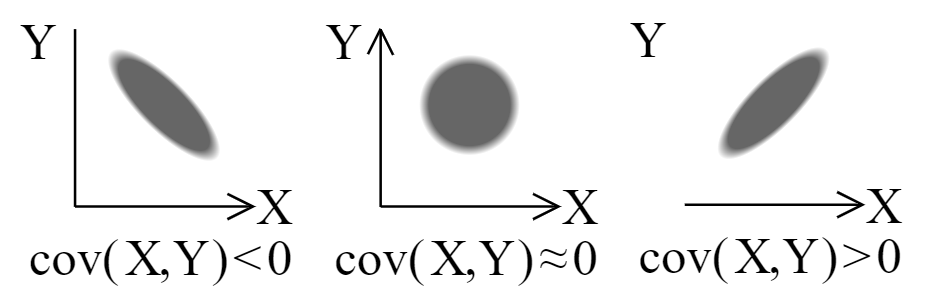
\includegraphics[width=8cm]{img/covarianza.png}
				  \vspace{-0.6cm}
		      \end{figure}
		\item Cálculo fundamental
		      \begin{align*}
			      V(X+ Y) & = E((X+Y)^2)- (E(X+Y))^2                              \\
			              & = E(X^2+2XY+Y^2)- (E(X)+E(Y))^2                       \\
			              & = E(X^2)+2E(XY)+E(Y^2)- (E(X))^2-2E(Y)E(X) - (E(Y))^2
		      \end{align*}
		      \[\implies \boxed{V(X+ Y) = V(X) + V(Y) + 2\cov{X, Y}}\]
		      Pero cuidado: $V(X-Y)=V(X) + V(Y) -2\cov{X, Y}$ \\
		      De forma más general:
		      \begin{align*}
			      V(aX+ bY) & = V(aX) + V(bY) + 2\cov{aX, bY}       \\
			                & = a^2V(X) + b^2V(Y) + 2ab\cov{aX, bY}
		      \end{align*}
		      \[\implies \boxed{V(aX+ bY)=a^2V(X) + b^2V(Y) + 2ab\cov{aX, bY}}\]
		\item Si $X$ e $Y$ son independientes $\implies \cov{X, Y}=0$
	\end{enumerate}
\end{obs}

\begin{defn}[coeficiente de correlación]
	Sean $X$ e $Y$ dos v.a.d., $\rho$ es su coeficiente de correlación $\ds \iff \boxed{\rho\defeq \frac{\cov{X, Y}}{\sqrt{V(X)\cdot V(Y)}}} \, \implies \rho\tex{ no tiene unidades y }\abs{\rho(X, Y)} \leq 1$.
\end{defn}
\begin{prop}[Desigualdad de Cauchy-Schwarz]
	Sean $X$ e $Y$ dos v.a.d.
	\[\implies E(X\cdot Y)^2 \leq E\left(X^2\right)\cdot E\left(Y^2\right)\]
	La igualdad se da cuando una variable es transformación lineal de la otra, i.e. $Y=aX+b$.
	\begin{dem}
		Definimos $W=sX+Y$, $W^2\geq 0$ con probabilidad 1.
		\begin{align*}
			\implies 0  \leq E\left(W^2\right) & =E\left((sX+Y)^2\right)=E\left(s^2X^2+Y^2+2sXY\right) \\
			& = s^2E\left(X^2\right)+E\left(Y^2\right)+2sE(XY)      \\
			& = E\left(X^2\right)\cdot s^2+2E(XY)\cdot s+E\left(Y^2\right)
		\end{align*}
		Vemos que el resultado es una parábola si se toma como función de $s$.\\
		Como $\forall s \in \R : E(X)\geq 0$ y $E\left(X^2\right)\geq 0$, sabemos que la parábola o bien toca el eje $X$ una única vez, o no lo hace nunca. Esto es equivalente a pedir que el valor del discriminante sea menor o igual que $0$.
		\[4E(XY)^2-4E\left(X^2\right)E\left(Y^2\right)\leq0 \implies E(XY)^2\leq E\left(X^2\right)E\left(Y^2\right)\]
	\end{dem}
\end{prop}
Por tanto, $\lbox{\cov{X, Y}^2} = E((X-E(X))(Y-E(Y)))^2 \leq \rbox{V(X)\cdot V(Y)\cdot\cov{X, Y}}$
\fecha{04/03/2024}
Además 
\fecha{05/03/2024}

\textbf{Dato:} $\ds (a_n)_{n=0}^\infty$ $\ds x\longmapsto\sum_{n=0}^\infty a_nx^n$ \\
Existe $R : \frac{1}{R}=\limsup_{n\to\infty}\abs{a_n}^{\sfrac{1}{n}} : \abs{x} < R \implies$ converge $\we \abs{x} > R \implies $ no converge.
\begin{ejem}
	\[ \sum_{n=0}^\infty \frac{x^n}{n!} = e^x \we \sum_{n=0}^\infty x^n = \frac{1}{1-x}, \abs{x}<1 \we \sum_{n=0}^m \binom{m}{n} x^n = (1+x)^m\]
\end{ejem}

\subsubsection{Funciones generatrices}
\[(a_n)_{n=0}^\infty \longleftrightarrow f(x)=\sum_{n=0}^\infty a_n x^n \implies \begin{cases}
		x\cdot f(x) \longleftrightarrow (0, a_0, \dots) \\
		x\cdot f'(x) \longleftrightarrow (0a_0, 1a_1, 2a_2, \dots)
	\end{cases}\]
\[f(x) \cdot g(x) = \sum_{n=0}^\infty a_n x^n \sum_{n=0}^\infty b_n x^n = \sum_{n=0}^\infty \left(\sum_{k=0}^n a_k b_{n-k}\right)x^n\]

\subsubsection{Funciones generatrices de probabilidad}
\begin{defn}
	Sea $X$ una variable aleatoria discreta que toma valores en $\{0, 1, 2, \dots\}$ donde $\forall j \geq 0 : p_j=P(X=j)$, $G_X(s)$ es su función generatriz de probabilidad
	\[\iff G_X(s)=\sum_{n=0}^\infty p_ns^n\]
\end{defn}
\begin{ejem}
	\begin{enumerate}
		\item[]
		\item $\ds X \sim \ber{p} \implies G_X(s)=(1-p)+ps$
		\item $\ds X \sim \bin{n, p} \implies G_X(s)= \sum_{j=1}^{n} \binom{n}{j} (1-p)^{n-j}(ps)^j = (1-p+ps)^n$
		\item $\ds X \sim \geom{p} \implies G_X(s)=\sum_{j=1}^\infty (1-p)^{j-1}ps^j = \frac{ps}{1-(1-p)s}$
		\item $\ds X \sim \poisson{\lambda} \implies G_X(s)=\sum_{j=0}^\infty e^{-\lambda}\frac{\lambda^j}{j!}s^j = e^{\lambda(s-1)}$
	\end{enumerate}
\end{ejem}

\textbf{¿Para qué?}
\begin{enumerate}
	\item Cálculo de momentos con $(p_n)_{n=0}^\infty$
	      \[ G_X(s)=\sum_{n=0}^\infty p_ns^n \implies G_X'(s) = \sum_{n=1}^{\infty} np_n s^{n-1} \implies G_X'(1) = \sum_{n=1}^{\infty} n p_n = E(X)\]
	      Si seguimos derivando, obetenemos
	      \[\implies G_X''(s)= \sum_{n=2}^{\infty} n(n-1) p_n s^{n-2} = \sum_{n=2}^{\infty} n^2 p_n s^{n-2} - \sum_{n=2}^{\infty} n p_n s^{n-2}\]
	      \[\implies G_X''(1) = \sum_{n=2}^{\infty} n^2 p_n - \sum_{n=2}^{\infty} n p_n = E(X^2) - E(X)\]
	      \[\implies V(X)=E(X^2) - E(X)^2 = G_X''(1) + G_X'(1)\left(1-G_X'(1)\right)\]
	      \begin{ejem}
		      \begin{enumerate}
			      \item[]
			      \item $\ds X\sim\ber{p} \implies G_X(s)=(1-p)+ps$
			            \[\implies G_X'(s)=p=E(X) \we G_X''(s)=0 \implies V(X)=p(1-p)\]
			      \item $\ds X\sim\bin{n, p} \implies G_X(s)=(1-p+ps)^n$ \[\implies G_X'(s)=n(1-p+ps)^{n-1}p \implies G_X'(1)=np=E(X)\]
			            \[\implies G_X''(s)=n(n-1)(\cdots)^{n-2}p^2 \implies G_X''(1)=n(n-1)p^2\]
			            \[\implies V(X)=n(n-1)p^2+np(1-np)=np(1-p)\]

		      \end{enumerate}
	      \end{ejem}
	\item Suma de independientes
\end{enumerate}
\begin{teo}
	Sean $X, Y$ dos v.a.d. independientes con valores en $\{0, 1, 2, \dots\}$ y con funciones generatrices de probabilidad $G_X(s), G_Y(s)$ respectivamente
	\[\implies G_{X+Y}(s)=G_X(s)\cdot G_Y(s)\]
	\begin{dem}
		\[G_{X+Y}(s)=\sum_{n=0}^\infty P(X+Y=n)s^n = \sum_{n=0}^\infty \left(\sum_{k=0}^n P(X=k \we Y=n-k)\right)s^n\]
		Por otro lado,
		\[\begin{aligned}G_X(s)\cdot G_Y(s) & = \left(\sum_{n=0}^\infty P(X=n)s^n\right)\left(\sum_{n=0}^\infty P(Y=n)s^n\right) \\
                                  & = \sum_{n=0}^\infty \left(\sum_{k=0}^n P(X=k)P(Y=n-k)\right)s^n\end{aligned}\implies G_{X+Y}(s)=G_X(s)\cdot G_Y(s)\]
		\hfill \qedsymbol\\
		Otra manera:
		\[G_X(s)=E(s^X) \we G_{X+Y}(s)=E\left(s^{X+Y}\right) = E\left(s^X\cdots^Y\right)=E(s^X)\cdot E(s^Y) = G_X(s)\cdot G_Y(s)\]
	\end{dem}
\end{teo}
\begin{cor}
	Sean $X_1, X_2, \dots, X_n$ v.a.d. independientes con valores en $\{0, 1, 2, \dots\}$ y con funciones generatrices de probabilidad $G_{X_1}(s), G_{X_2}(s), \dots, G_{X_n}(s)$ respectivamente
	\[\implies G_{X_1+X_2+\dots+X_n}(s)=\prod_{i=1}^{n} G_{X_i}(s)\]
	Si las $X_i$ son ``idénticas'' $\ds \implies G_{X_1+X_2+\dots+X_n}(s)=\left(G_{X_1}(s)\right)^n$
\end{cor}
\fecha{06/03/2024}

\begin{teo}[Unicidad]
	Sean $X, Y$ dos v.a.d. con valores en $\{0, 1, 2, \dots\}$ y con funciones generatrices de probabilidad $G_X(s), G_Y(s)$ respectivamente
	\[\implies G_X(s)=G_Y(s) \iff \forall n\geq 0 : P(X=n)=P(Y=n)\]
\end{teo}

\begin{ejem}
	Sean $X\sim\poisson{\lambda} \we Y\sim\poisson{\mu}$ independientes con $\lambda, \mu > 0$. Definimos $Z=X+Y$.
	\[\implies \forall x \geq 0 : P(Z=k) = P(X+Y=k)= \sum_{j=0}^{k} P(X=j \we Y=k-j) = \cdots\]
	Pero, a través de funciones generatrices obtenemos:
	\[G_X(s)=e^{\lambda(s-1)} \we G_Y(s)=e^{\mu(s-1)} \implies G_{Z}(s)=e^{(\lambda+\mu)(s-1)}\implies Z\sim\poisson{\lambda+\mu}\]
\end{ejem}

\begin{ejem}
	\begin{enumerate}
		\item []
		\item Sean $I_1, I_2, \dots, I_n$ v.a.d. independientes con $\forall k \in \N_n : I_k\sim\ber{p}$ y definimos $Z=I_1+I_2+\cdots+I_n$.
		      \[\implies G_Z(s)={\left[(1-p)+ps\right]}^n \implies Z \sim \bin{n, p}\]
		\item Sean $X \sim \bin{n, p} \we Y\sim \poisson{\lambda}$ independientes y definimos $Z=X+Y$.
		      \[\implies G_Z(s)={\left((1-p)+ps\right)}^n\cdot e^{\lambda(s-1)}\]
	\end{enumerate}
\end{ejem}

\fecha{11/03/2024}

